\documentclass[oneside]{hcmut-report}

\usepackage{codespace}
\usepackage[dvipsnames]{xcolor}
\usepackage[most]{tcolorbox}
\usepackage{array,booktabs,tabularx,multirow}
\usepackage{enumitem}
\usepackage{caption,float}
\usepackage[export]{adjustbox}

\geometry{paper=a4paper,left=2cm,right=2cm,top=1cm,bottom=1cm,includeheadfoot,headheight=34.8pt,headsep=12pt,footskip=30pt,asymmetric}
\definecolor{myblue}{RGB}{33,102,172}
\newtcolorbox{importantbox}{colback=Green!8,colframe=ForestGreen!80!black,boxrule=0.8pt,arc=1mm,left=3mm,right=3mm,top=1mm,bottom=1mm}

\coursename{CO5085 -- Deep Learning and Its Applications in Computer Vision}
\reporttype{Assignment A1 Report}
\title{CNN vs Transformer on CIFAR-100}
\advisor{Dr. Le Thanh Sach and Dr. Nguyen Quoc Minh}
\stuname{Dinh Hoang Duy Khanh \quad 2670306}
\reportplace{Ho Chi Minh City}
\reporttime{November 2026}
\setcounter{tocdepth}{2}

\newcommand{\reportleftheader}{%
  \bfseries
  \begin{tabular}{rl}
    \begin{picture}(25pt,15pt)
      \put(0,-8pt){
\includegraphics[width=20pt]{graphics/hcmut.png}}
    \end{picture}
    \begin{tabular}{l}
      \ttfamily Ho Chi Minh City University of Technology \\[-5pt]
      \ttfamily Faculty of Computer Science and Engineering \\
    \end{tabular}
  \end{tabular}%
}
\fancypagestyle{plain}{%
  \fancyhf{}%
  \fancyhead[L]{\reportleftheader}
  \fancyfoot[L]{\raisebox{3pt}{\ttfamily CO5085 Assignment A1 -- Semester HK261}}
  \fancyfoot[R]{\raisebox{3pt}{\ttfamily Page \thepage/\pageref{LastPage}}}
  \renewcommand{\headrulewidth}{0.4pt}%
  \renewcommand{\footrulewidth}{0.4pt}%
}
\AtBeginDocument{\pagestyle{plain}}

\begin{document}
\begin{titlepage}
\begin{center}
VIETNAM NATIONAL UNIVERSITY -- HO CHI MINH CITY \\
HO CHI MINH CITY UNIVERSITY OF TECHNOLOGY \\
FACULTY OF COMPUTER SCIENCE AND ENGINEERING
\end{center}
\vspace{0.5cm}
\begin{figure}[h!]
\centering
\includegraphics[width=4.5cm]{graphics/hcmut.png}
\end{figure}
\vspace{0.4cm}
\begin{center}
\begin{tabular}{c}
\multicolumn{1}{c}{\textbf{\Large CO5085 ASSIGNMENT A1 REPORT}}\\
~~\\ \hline \\[-2pt]
\textbf{\large CNN VS TRANSFORMER ON CIFAR-100}\\[4pt]
\textbf{\large \textit{Group: Traiblazer}}\\[-2pt]
\hline
\end{tabular}
\end{center}
\vspace{0.9cm}
\begin{table}[h]\centering
\begin{tabular}{rll}
\textbf{Instructors:} & Dr. Le Thanh Sach & \\
& Dr. Nguyen Quoc Minh & \\[8pt]
\textbf{Student:} & Dinh Hoang Duy Khanh & 2670306 \\
\end{tabular}
\end{table}
\vfill
\begin{center}{\footnotesize \textit{Ho Chi Minh City, November 2026}}\end{center}
\end{titlepage}

\section*{Member List and Workload}
\addcontentsline{toc}{section}{Member List and Workload}
\begin{center}\small
\begin{tabular}{|c|p{3.2cm}|c|p{4.9cm}|c|}\hline
\textbf{No.} & \textbf{Name} & \textbf{Student ID} & \textbf{Main responsibilities} & \textbf{Contribution} \\\hline
1 & Dinh Hoang Duy Khanh & 2670306 & Select the dataset, implement the eight A1 experiments, run training, create figures, update GitHub Pages, and write this report. & 100\% \\\hline
\end{tabular}
\end{center}
\clearpage
\begingroup\footnotesize\tableofcontents\endgroup
\clearpage

\section*{Introduction and Assignment Goal}
\addcontentsline{toc}{section}{Introduction and Assignment Goal}
Assignment A1 asks for a fair comparison between a CNN and a Transformer on a public image dataset that is larger and harder than the E1 dataset. The comparison must include random initialization and ImageNet pretraining. For each pretrained model, it must include three choices: train the classifier head only, train part of the backbone, and train all layers. It must also report accuracy or F1, training cost, and error analysis.

This project uses CIFAR-100. The code compares ResNet-18, a CNN, with Swin-T, a hierarchical vision Transformer. There are eight experiments: four for each family. Every experiment uses the same train-validation split and the same three-epoch budget. Validation accuracy selects one configuration. The untouched official test set is used only after that selection. This rule prevents a test result from deciding which model looks best.

\begin{importantbox}
\textbf{Main measured result.} The validation winner is ImageNet-pretrained Swin-T with full fine-tuning. It obtains validation accuracy 0.8281. One final run on the official CIFAR-100 test set gives accuracy 0.8173 and macro-F1 0.8162. These numbers are measured by \texttt{A1/run\_a1.py}; they are not estimated values.
\end{importantbox}

\clearpage
\subsection*{A1 requirement checklist}
\addcontentsline{toc}{subsection}{A1 requirement checklist}
\begin{tabularx}{\textwidth}{>{\bfseries}p{3.4cm}X}\toprule
\textbf{Assignment requirement} & \textbf{Evidence in this project} \\\midrule
Large public image dataset & CIFAR-100 has 50,000 official training images, 10,000 official test images, and 100 fine classes. \\
CNN and Transformer & ResNet-18 is the CNN; Swin-T is the Transformer. \\
Scratch and pretrained & Both model families have a random-initialized \texttt{scratch} run and three ImageNet-pretrained runs. \\
Three freeze choices & \texttt{head}, \texttt{partial}, and \texttt{full} are implemented and measured for both families. \\
Metrics and cost & Table~\ref{tab:all-results} gives validation accuracy, trainable parameters, time, and peak GPU memory. \\
Error analysis & A 20-superclass confusion matrix and real wrong-prediction images come from the selected model's one final test run. \\
Reproducible delivery & Code, JSON output, figures, this PDF, README, and a GitHub Pages A1 card are in the same repository. \\\bottomrule
\end{tabularx}

\clearpage
\section{CIFAR-100 Dataset and Protocol}
\subsection{Why this dataset is suitable}
CIFAR-100 contains 60,000 colour images of size $32\times32$. It has 100 fine classes such as \textit{apple}, \textit{camel}, and \textit{tulip}. Each fine class has 500 official training images and 100 official test images. The 100 fine classes are also grouped into 20 larger superclasses. For example, several animal classes belong to the same broad group. The large number of fine classes makes the task much harder than CIFAR-10 or Fashion-MNIST.

The original CIFAR page is the dataset source~[1]. It describes the data and asks users to cite the technical report. The original public page does not state an explicit licence. Therefore, this report does not claim an MIT or commercial licence. The data and pretrained weights are used only for this educational coursework, with their source and limitations stated clearly. The local loader uses the public \texttt{uoft-cs/cifar100} Hugging Face copy for reliable automatic downloading; it keeps the original train/test partition.

\subsection{Split, loader, and augmentation}
The official 50,000-image training partition is split with seed 42. For every one of the 100 fine classes, the code shuffles its 500 indices, places 400 images in training and 100 in validation, and then joins the classes. This makes the split exactly balanced: 40,000 training images and 10,000 validation images. The official 10,000-image test partition is not mixed with either set.

The model expects $96\times96$ RGB input. A resize changes the tensor size but does not invent new visual information; it makes the input shape practical for the ImageNet-pretrained models. During training only, \texttt{RandomCrop} with padding and \texttt{RandomHorizontalFlip} create slightly changed versions of an image. Validation and test use only resize and normalization, so their measurements are repeatable. The ImageNet channel mean $(0.485,0.456,0.406)$ and standard deviation $(0.229,0.224,0.225)$ are used for all eight runs. This keeps the input rule the same for CNN and Transformer.

\begin{figure}[H]\centering
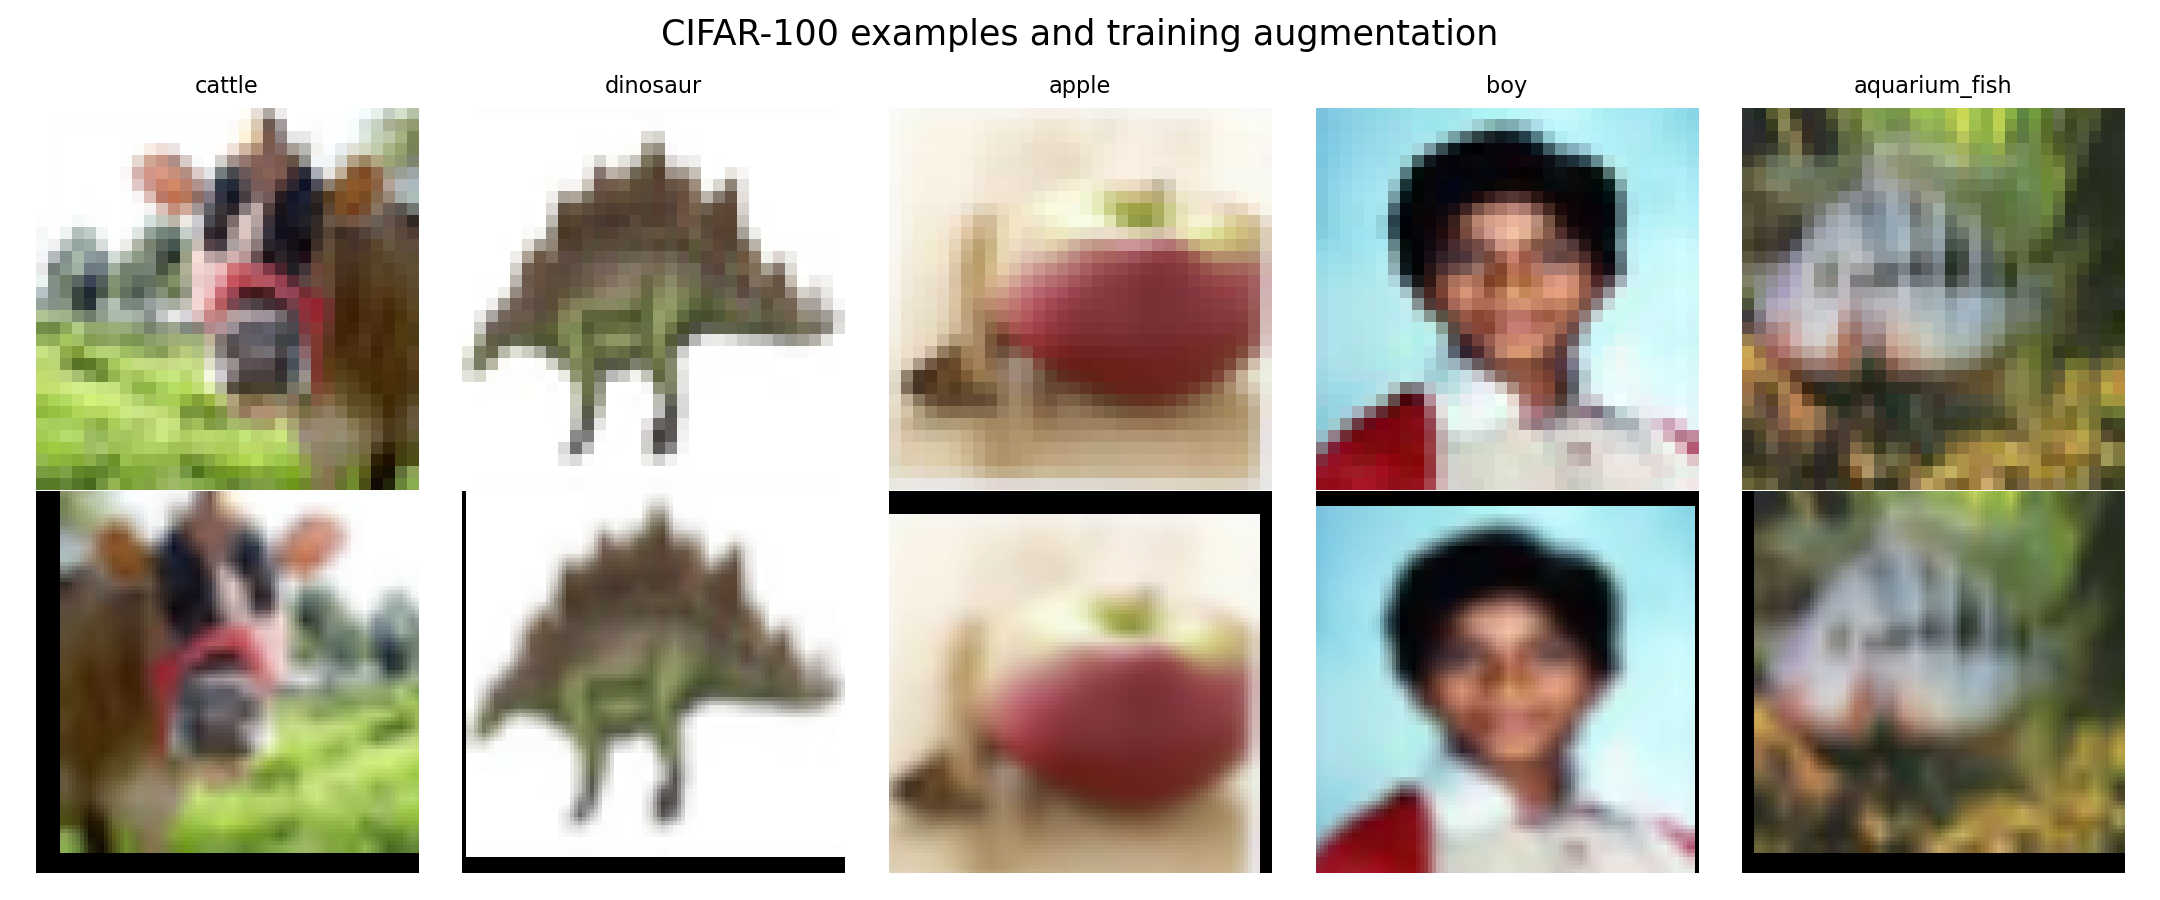
\includegraphics[width=0.95\textwidth]{images/a1_01_augmentation.png}
\caption{Five CIFAR-100 examples (top) and the random training augmentation applied to them (bottom). The random changes are used for training only.}\label{fig:augmentation}
\end{figure}

\subsection{Data representation and evaluation metrics}
One input batch is $X\in\mathbb{R}^{B\times3\times96\times96}$, where $B=64$, 3 is the RGB channel count, and 96 is height and width after resize. The label $y$ is an integer from 0 to 99. A model returns 100 logits $z=(z_1,\ldots,z_{100})$. Softmax changes logits into probabilities:
\[
p_i=\frac{\exp(z_i)}{\sum_{j=1}^{100}\exp(z_j)}.
\]
For true label $y$, cross-entropy loss is
\[
\mathcal{L}=-\log(p_y).
\]
In the code, \texttt{nn.CrossEntropyLoss()} receives logits directly and calculates this stable softmax-loss expression internally. A prediction is the class with the largest logit. Accuracy is
\[
\mathrm{accuracy}=\frac{\text{number of correct predictions}}{\text{number of evaluated images}}.
\]
Macro-F1 calculates F1 separately for each of the 100 classes and then takes their unweighted mean. It gives every class equal importance, which is useful when a class-specific failure could be hidden by a single average accuracy.

\clearpage
\section{ResNet-18 and Swin-T Theory}
\subsection{ResNet-18: the CNN model}
ResNet-18 is a convolutional neural network with residual blocks~[2]. A normal block learns a transformation $F(x,W)$ of its input $x$. A residual block adds the input back before the activation:
\[
y=\mathrm{ReLU}(F(x,W)+x).
\]
The shortcut $+x$ gives a direct path for information and gradients. In simple words, a layer can learn only the change it needs instead of rebuilding the whole representation. Convolutions read small nearby pixel regions, so ResNet naturally learns local edges, colours, and textures. After several stages, a final linear layer converts learned features into 100 class scores.

The torchvision ResNet-18 starts with an ImageNet classifier head containing 1,000 outputs. The code replaces that head with \texttt{nn.Linear(..., 100)}. This replacement is necessary because CIFAR-100 has 100 classes. In a frozen-backbone run, BatchNorm layers without trainable parameters are kept in evaluation mode. Their running mean and variance then remain frozen as well.

\subsection{Swin-T: the Transformer model}
Swin-T is a hierarchical vision Transformer based on shifted local windows~[3]. First, the image is divided into non-overlapping patches. A patch is flattened and projected to a token vector:
\[
t=W_p\,\mathrm{flatten}(x_{\mathrm{patch}})+b_p.
\]
The model forms query, key, and value matrices from tokens $T$:
\[
Q=TW_Q,\qquad K=TW_K,\qquad V=TW_V.
\]
Inside one local window, scaled dot-product attention is
\[
\mathrm{Attention}(Q,K,V)=\mathrm{softmax}\left(\frac{QK^T}{\sqrt{d_k}}\right)V.
\]
The product $QK^T$ compares one token with other tokens. Softmax converts comparisons to weights, and the weighted sum of $V$ shares useful information. Using local windows avoids computing attention across every image patch at once. In the next block, shifted windows change the window boundaries, so information can pass between neighboring windows. This is the main Swin idea: it keeps attention efficient while building a larger visual context across stages.

Like ResNet, Swin-T has a final ImageNet head with 1,000 outputs. The code replaces \texttt{model.head} with a 100-output linear layer. Swin-T has more parameters than ResNet-18 and needs more memory/time, but it can use relations between patches through attention.

\subsection{Why pretrained weights matter}
ImageNet pretraining gives parameters $\theta_0$ that have already learned general visual patterns from a large image dataset. A random model instead starts at random $\theta_{\mathrm{random}}$. During fine-tuning, gradient-based optimization updates trainable parameters:
\[
\theta\leftarrow\theta-\eta\nabla_\theta\mathcal{L},
\]
where $\eta$ is the learning rate. AdamW implements a more stable version of this update with moving averages and weight decay, but the idea remains: reduce loss by moving parameters in the opposite direction of its gradient.

Pretraining does not solve the new task automatically because ImageNet has 1,000 different labels. The new 100-class head must learn CIFAR-100 labels. The experiment tests how much of the pretrained backbone should change while learning that head.

\clearpage
\section{Transfer Learning and Freeze Modes}
\subsection{The four configurations}
Each model family uses four configurations. The same data, split, batch size, and epoch count are used in every configuration. The mode changes only parameter initialization and which parameters receive gradients.

\begin{table}[H]\centering\small
\caption{A1 experiment matrix. \texttt{partial} means the last feature stage plus the new classifier head.}\label{tab:matrix}
\begin{tabularx}{\textwidth}{>{\ttfamily}l>{\ttfamily}lX}\toprule
\textbf{Family} & \textbf{Mode} & \textbf{Initialization and trainable part} \\\midrule
cnn & scratch & ResNet-18 random initialization; all parameters train. \\
cnn & head & ImageNet ResNet-18; only \texttt{fc} classifier head trains. \\
cnn & partial & ImageNet ResNet-18; \texttt{layer4} and \texttt{fc} train. \\
cnn & full & ImageNet ResNet-18; every parameter trains. \\
transformer & scratch & Swin-T random initialization; all parameters train. \\
transformer & head & ImageNet Swin-T; only \texttt{head} classifier trains. \\
transformer & partial & ImageNet Swin-T; final \texttt{features} stage and \texttt{head} train. \\
transformer & full & ImageNet Swin-T; every parameter trains. \\\bottomrule
\end{tabularx}
\end{table}

\subsection{What freezing changes}
For \texttt{head}, the backbone weights stay fixed. Only the new classifier learns. This is fast and uses little GPU memory because few gradients and optimizer states are stored. It works well when pretrained features already match the new images, but it cannot change the backbone if CIFAR-100 needs different features.

For \texttt{partial}, the early stages remain fixed and only the final stage is allowed to adapt. This is a middle choice: low-level edges and basic shapes are reused, while higher-level class features can change. It costs more than head-only training but less than full fine-tuning.

For \texttt{full}, every pretrained parameter receives gradients. It has the greatest capacity to adapt, but is also the most expensive. It may need a smaller learning rate so good pretrained features are not changed too abruptly. Here head-only uses learning rate 0.001, scratch and partial use 0.0003, and full uses 0.0001. These rates are written explicitly in the JSON result file.

\subsection{Experiment Algorithm}
The following steps correspond directly to \texttt{A1/run\_a1.py}.
\begin{enumerate}[leftmargin=8mm]
  \item Set seed 42. Load CIFAR-100 train and test partitions, then make 400 training and 100 validation indices for every fine class.
  \item Build a training loader with resize, random crop, random flip, tensor conversion, and normalization. Build validation and test loaders without random augmentation.
  \item For one experiment row, call \texttt{build\_model}. It loads ResNet-18 or Swin-T, optionally loads ImageNet weights, replaces the classifier by 100 outputs, and applies the selected freeze mode.
  \item Count parameters with \texttt{requires\_grad=True}. Start the timer and reset GPU peak-memory statistics.
  \item For each of three epochs, read a batch, move images and labels to CUDA, call the model, and get 100 logits per image.
  \item Compute \texttt{CrossEntropyLoss}. Clear old gradients with \texttt{zero\_grad()}, call \texttt{loss.backward()}, then call \texttt{optimizer.step()}.
  \item Switch to evaluation mode and calculate validation loss and accuracy without gradients. Keep a CPU copy of the weights when validation accuracy improves.
  \item Repeat Steps 3--7 for all eight rows. Do not inspect the official test partition while choosing a row.
  \item Select the largest validation accuracy using \texttt{select\_best\_experiment}. Load its saved best-validation weights and evaluate the official test partition only after selection.
  \item Save JSON metrics and figures: augmentation examples, learning curves, cost comparison, a 20-superclass confusion matrix, and wrong-prediction examples.
\end{enumerate}

\clearpage
\section{Measured Results and Discussion}
\subsection{Execution environment}
All numbers in this section come from one executed script on an NVIDIA GeForce RTX 3050 Ti Laptop GPU. Inputs are $96\times96$, batch size is 64, and every row trains for three epochs. The output file \texttt{reports/a1\_results.json} stores the unrounded values. Time measures the three training epochs and three validation passes for one configuration. Peak GPU memory is measured by PyTorch during that configuration.

\begin{table}[H]\centering\small
\caption{All eight measured validation experiments. The highest validation accuracy is bold.}\label{tab:all-results}
\resizebox{\textwidth}{!}{%
\begin{tabular}{llrrrr}
\toprule
\textbf{Family} & \textbf{Mode} & \textbf{Validation accuracy} & \textbf{Trainable parameters} & \textbf{Time (s)} & \textbf{Peak memory (MB)} \\
\midrule
ResNet-18 & scratch & 0.3689 & 11,227,812 & 147.7 & 434.2 \\
ResNet-18 & head & 0.5698 & 51,300 & 35.2 & 138.7 \\
ResNet-18 & partial & 0.6930 & 8,445,028 & 48.2 & 235.2 \\
ResNet-18 & full & 0.7441 & 11,227,812 & 91.3 & 434.2 \\
Swin-T & scratch & 0.1971 & 27,596,254 & 470.4 & 1,826.2 \\
Swin-T & head & 0.7076 & 76,900 & 169.1 & 330.4 \\
Swin-T & partial & 0.7573 & 14,260,756 & 234.8 & 493.4 \\
Swin-T & full & \textbf{0.8281} & 27,596,254 & 470.4 & 1,826.5 \\
\bottomrule
\end{tabular}}
\end{table}

\begin{figure}[H]\centering
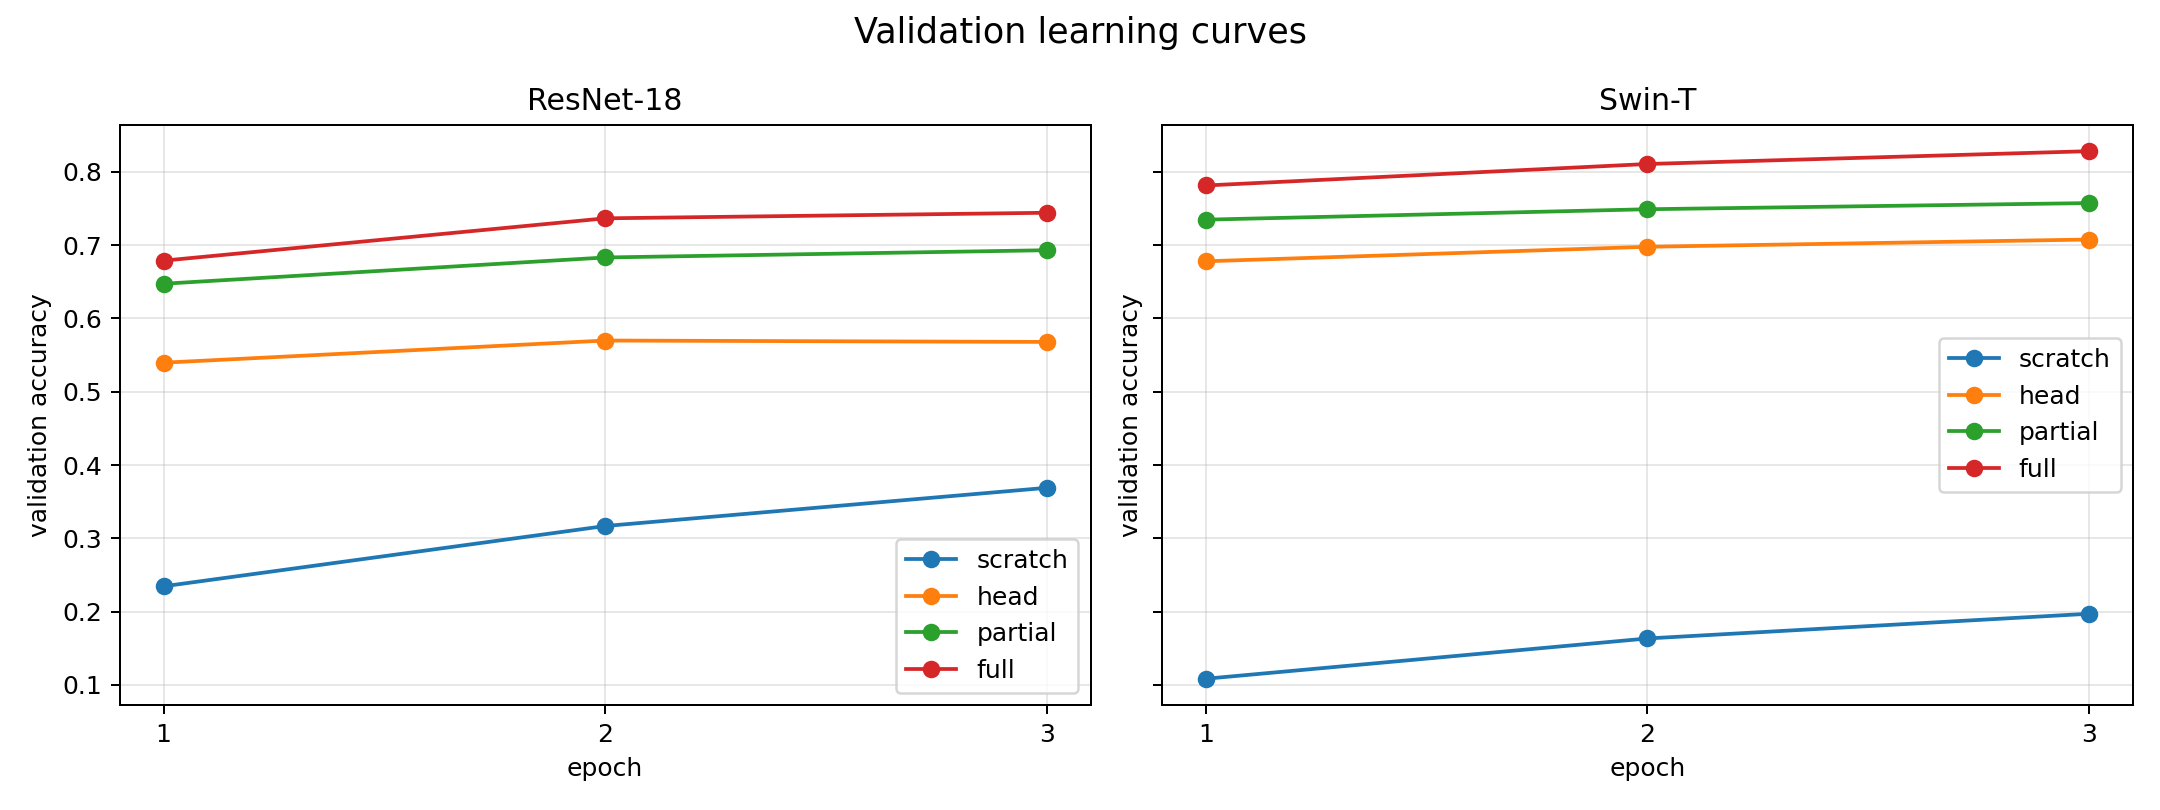
\includegraphics[width=0.95\textwidth]{images/a1_02_learning_curves.png}
\caption{Validation accuracy after each epoch. Each panel compares the four freeze modes inside one model family.}\label{fig:curves}
\end{figure}

The two scratch results are low: ResNet-18 reaches 0.3689 and Swin-T reaches 0.1971. This does not prove that a Transformer is always worse. It shows that a larger Transformer trained from random weights needs more optimization time and possibly a different schedule. In this controlled three-epoch setting, ResNet's local convolution prior learns CIFAR-100 faster from scratch.

Pretraining changes the result strongly. Head-only training improves ResNet-18 from 0.3689 to 0.5698 and Swin-T from 0.1971 to 0.7076. Swin-T head-only is slower than ResNet head-only because it still runs the complete Transformer forward pass, but it needs only 76,900 trainable parameters and 330.4 MB peak memory. This can be useful when GPU memory is limited.

\subsection{Freeze comparison and training cost}
For ResNet-18, full fine-tuning is best at 0.7441. Partial fine-tuning gives 0.6930 while training 8.45 million parameters instead of 11.23 million. Head-only is cheapest at 35.2 seconds but loses accuracy. This gives a simple trade-off: select head-only when a fast baseline is enough, partial when reducing cost matters, and full when the additional accuracy is worth the cost.

For Swin-T, the same order appears: head-only gives 0.7076, partial gives 0.7573, and full gives 0.8281. Full fine-tuning takes 470.4 seconds and about 1.83 GB peak memory. It is around five times the ResNet full-training time, so its higher accuracy has a real cost. The selected configuration is suitable for the available GPU, but it would be less practical on a CPU-only machine.

\begin{figure}[H]\centering
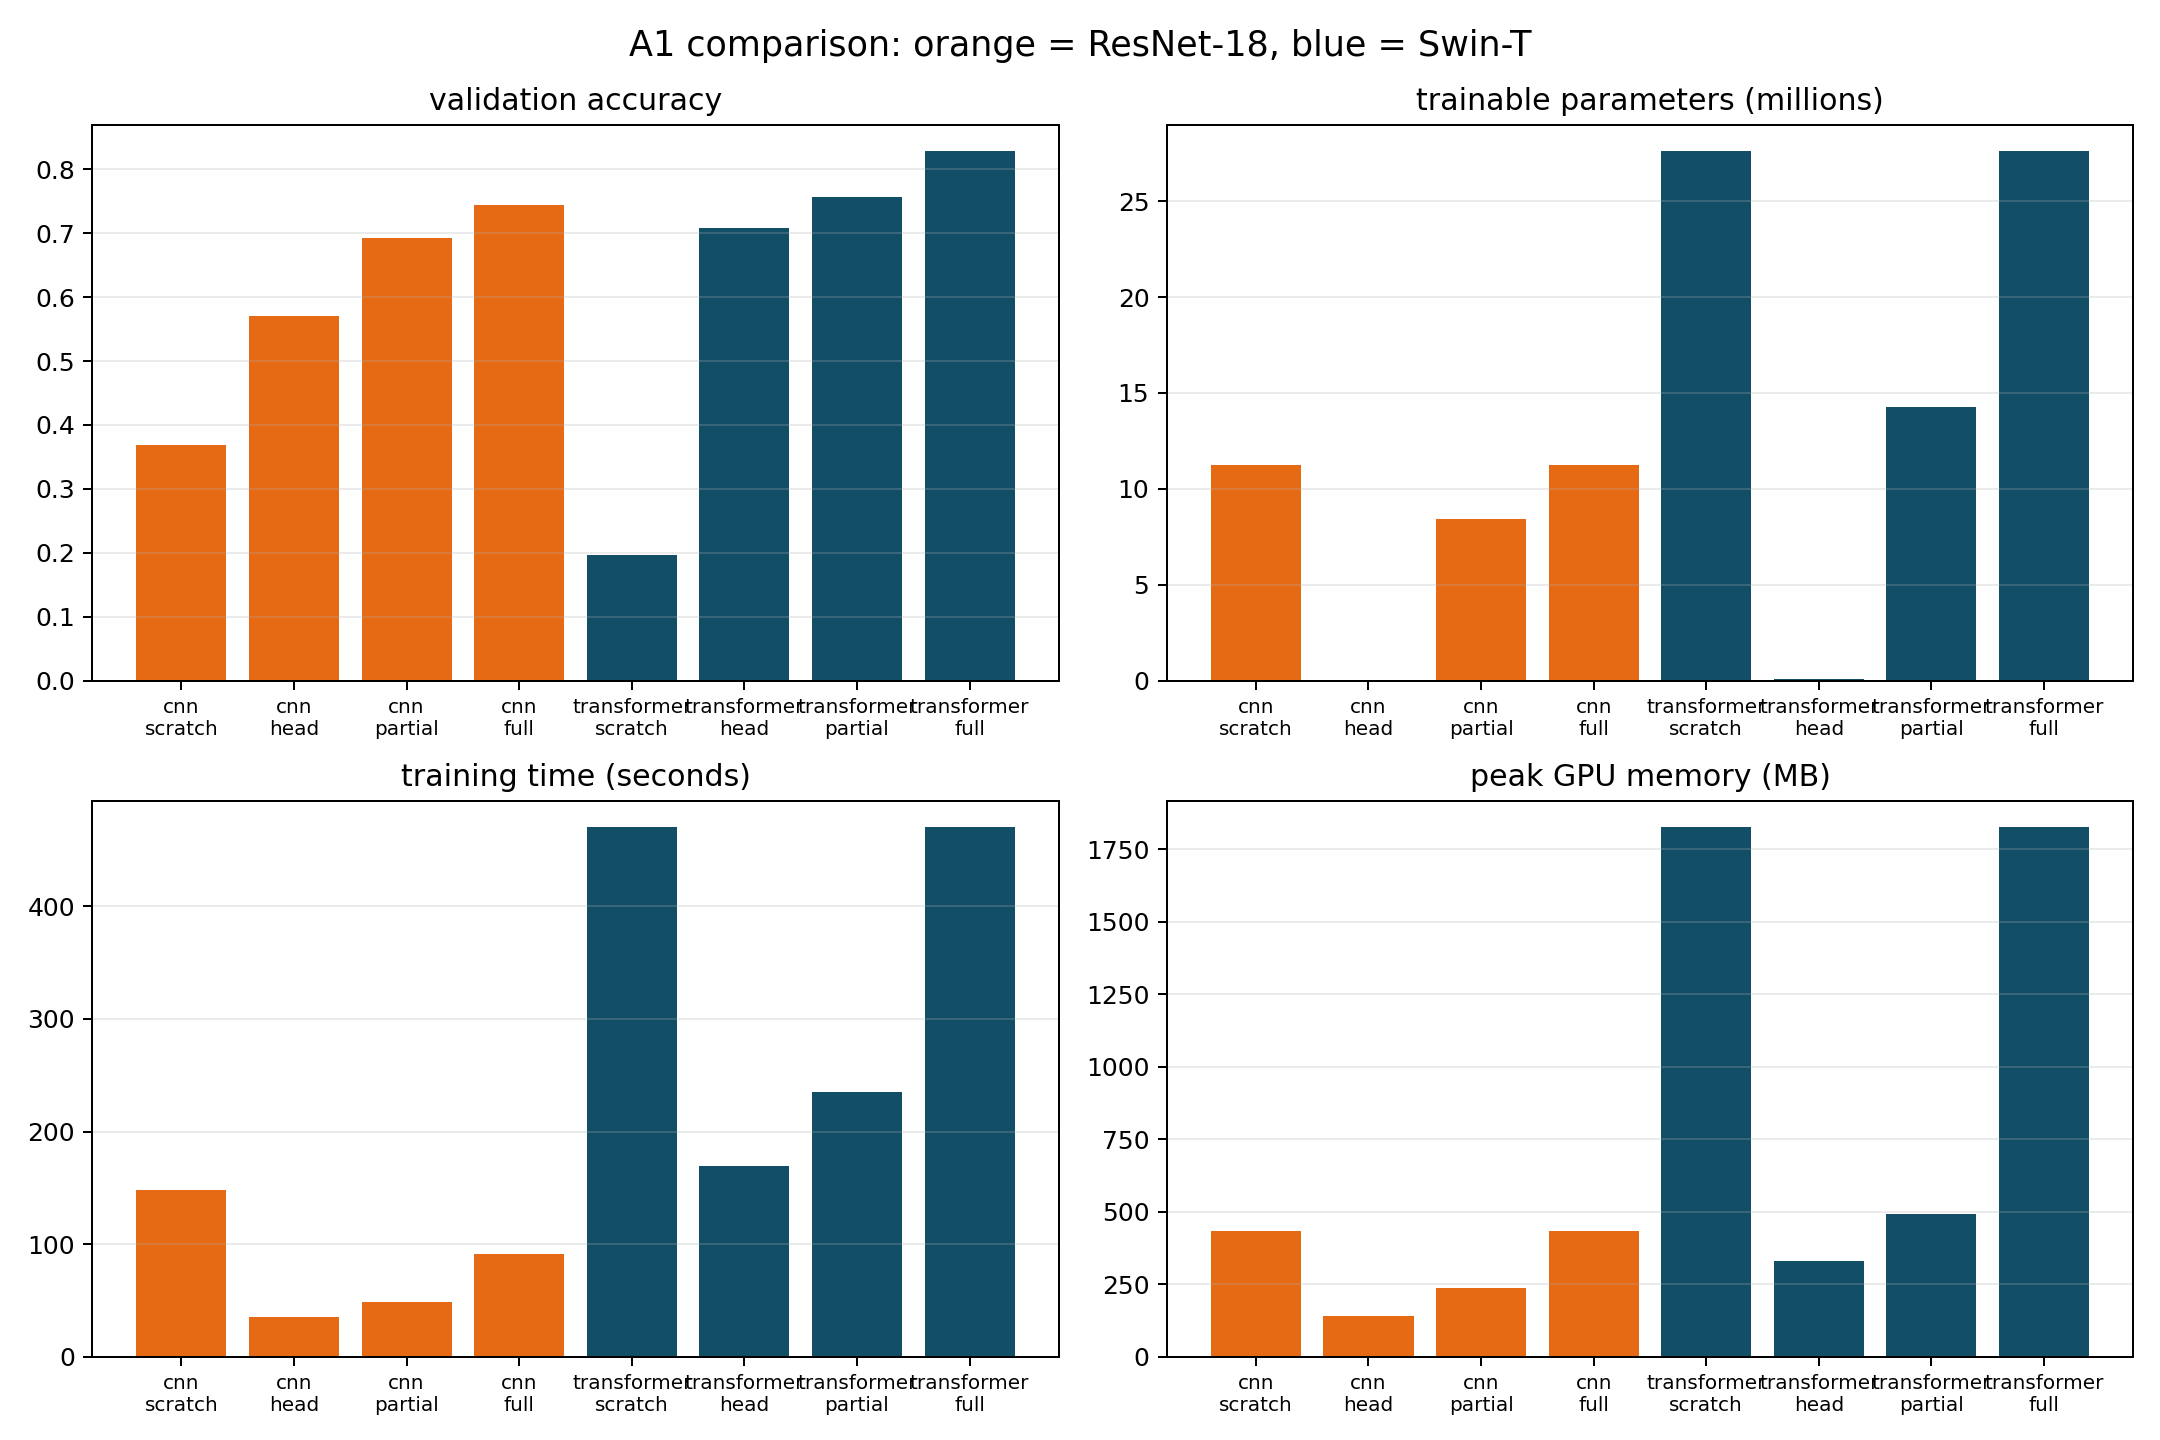
\includegraphics[width=0.95\textwidth]{images/a1_03_comparison.png}
\caption{Validation accuracy, trainable parameters, training time, and peak GPU memory for all eight experiments. Orange bars are ResNet-18; blue bars are Swin-T.}\label{fig:comparison}
\end{figure}

\subsection{Official test evaluation after validation selection}
The largest validation accuracy is Swin-T full fine-tune at 0.8281. The saved checkpoint from the best validation epoch is evaluated on the untouched official test partition only after validation selects it. The recorded final test metrics are in Table~\ref{tab:test}. No other configuration receives a test metric for model selection, because comparing many test metrics and choosing the largest one would leak test information into selection.

\begin{table}[H]\centering
\caption{One official test evaluation after validation selection.}\label{tab:test}
\begin{tabular}{lrr}\toprule
\textbf{Selected model} & \textbf{Test accuracy} & \textbf{Test macro-F1} \\\midrule
Swin-T, ImageNet pretrained, full fine-tune & \textbf{0.8173} & \textbf{0.8162} \\\bottomrule
\end{tabular}
\end{table}

After the recorded sweep, the already-selected Swin-T full configuration was run again only to regenerate the numbered confusion matrix in Figure~\ref{fig:confusion}. That post-selection reproduction gave test accuracy 0.8140, compared with 0.8173 in Table~\ref{tab:test}. The 0.0033 difference is reported openly: GPU training with parallel data loading can vary slightly between runs. This extra run did not choose or change the selected configuration.

\clearpage
\section{Error Analysis, Limitations, and Reproduction}
\subsection{Confusion matrix and wrong predictions}
The selected model predicts 100 fine classes. A $100\times100$ confusion matrix would be hard to read in a report, so Figure~\ref{fig:confusion} groups true and predicted fine labels into CIFAR-100's 20 official superclasses. Each row is normalized, so the dark diagonal means that a broad group is usually predicted correctly. It is only a readability summary; the model itself still predicts the 100 fine labels. This figure uses the transparent post-selection reproduction described in Section~4.3; it is not used to select a model.

Figure~\ref{fig:errors} shows 12 real wrong predictions from the final test run. Several pairs have visual or semantic similarity: mountain versus road, cloud versus sea, tulip versus orchid, camel versus crocodile, and rabbit versus kangaroo. Some errors also show the basic problem of CIFAR-100: a $32\times32$ source image can contain little detail. Upsizing to $96\times96$ helps the network interface but cannot add missing pixels.

\begin{figure}[H]\centering
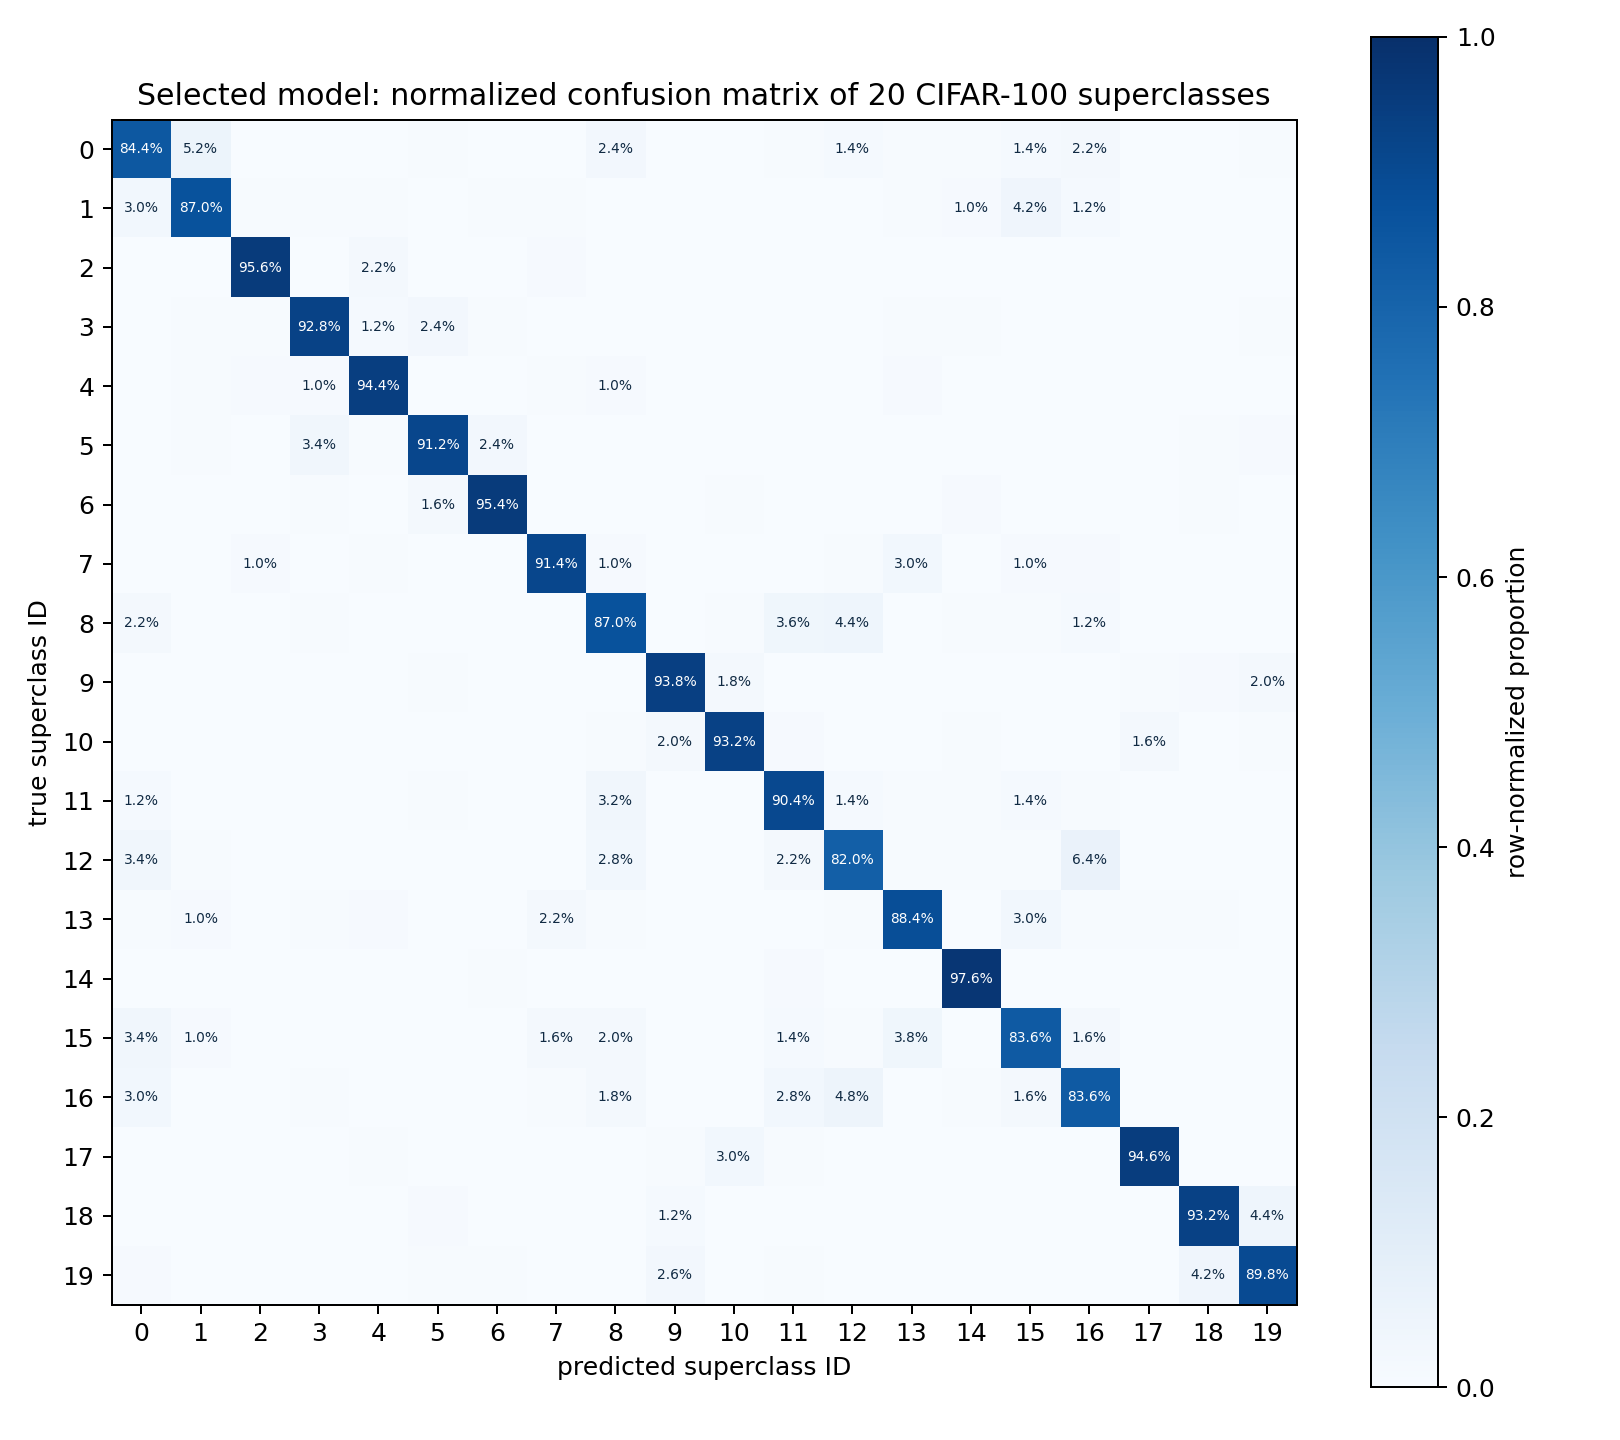
\includegraphics[width=0.78\textwidth]{images/a1_04_coarse_confusion_matrix.png}
\caption{Row-normalized confusion matrix of the 20 CIFAR-100 superclasses for the selected model. Cells at or above 1\% show their percentage; smaller cells are blank to keep the figure readable.}\label{fig:confusion}
\end{figure}
\begin{figure}[H]\centering
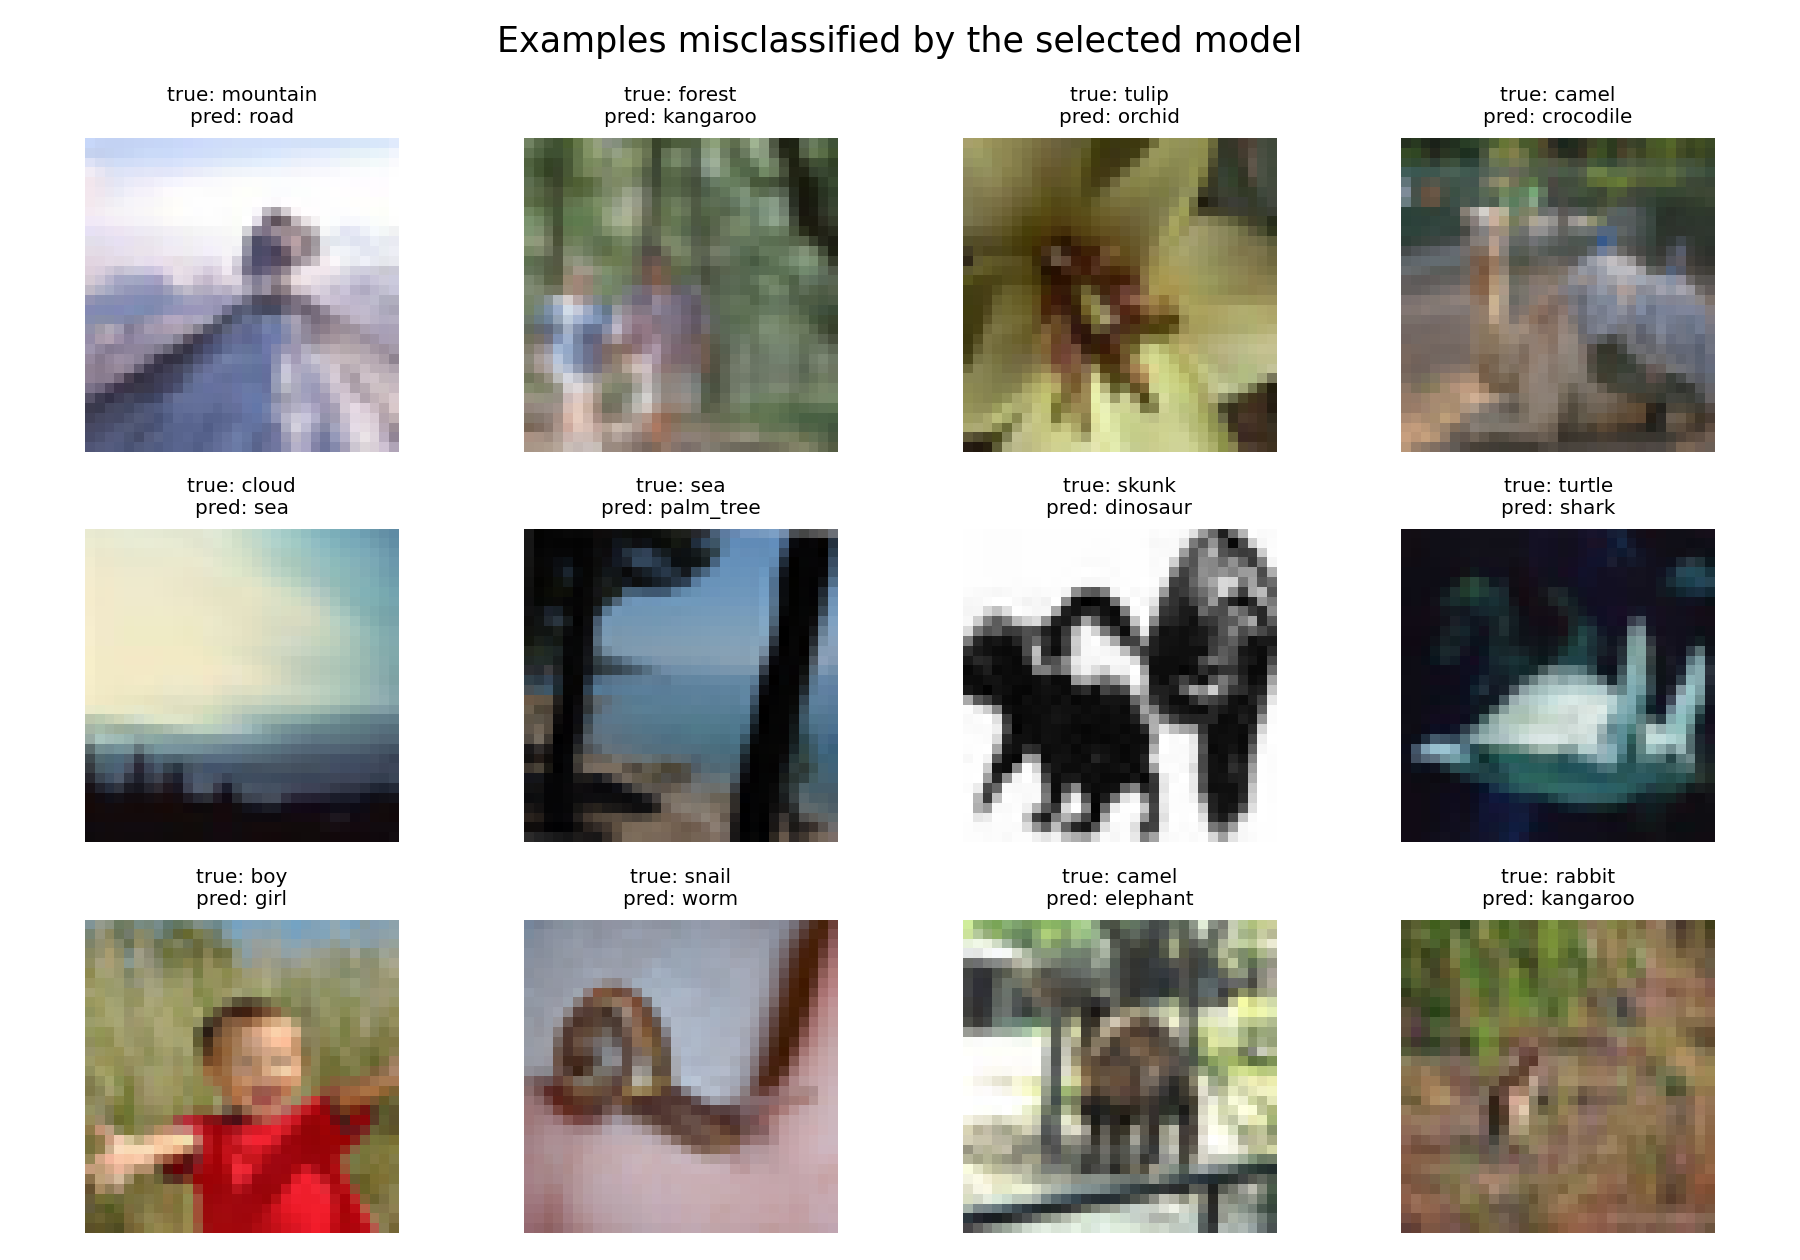
\includegraphics[width=0.94\textwidth]{images/a1_05_error_examples.png}
\caption{Twelve wrong fine-class predictions from the selected model's one final test evaluation.}\label{fig:errors}
\end{figure}

\subsection{Limitations}
This is a clear A1 comparison, but it is not a maximum-performance CIFAR-100 study. First, every experiment has only three epochs. The low scratch results, especially Swin-T, would likely improve with a longer training schedule, a learning-rate schedule, and several random seeds. Second, CIFAR-100 source images are only $32\times32$; resizing to $96\times96$ is required for a practical pretrained-model interface but does not create new detail. Third, the results come from one GPU and one seed. Time and memory may change on another machine. Fourth, the source dataset page does not give an explicit licence, so this work should remain educational unless its terms are checked again for a different use.

\subsection{How to reproduce}
Install packages from the repository root and run:
\begin{verbatim}
pip install -r requirements.txt
python -m A1.run_a1
\end{verbatim}
The first run downloads the public dataset and torchvision ImageNet weights. The script saves \texttt{reports/a1\_results.json} and five PNG files under \texttt{reports/figures/}. The A1 README explains the files in beginner-friendly order. The project page links directly to the code and this PDF.

\section{Conclusion}
This assignment compares two visual model families under the same CIFAR-100 split. With three epochs of random initialization, ResNet-18 learns faster than Swin-T. ImageNet pretraining improves both models substantially. For pretrained models, opening more layers increases both accuracy and cost. Swin-T full fine-tuning gives the best validation accuracy, 0.8281, and the selected model gives 0.8173 test accuracy with macro-F1 0.8162. ResNet-18 remains a smaller and faster alternative, while Swin-T gives the strongest measured result on the available GPU.

The code keeps the learning steps visible: make a balanced split, load and augment images, build a model, choose trainable parameters, calculate cross-entropy, call backward propagation, evaluate validation data, then test one selected model. This makes the project suitable for a new learner while still covering the complete A1 protocol.

\clearpage
\section*{References}
\addcontentsline{toc}{section}{References}
\begin{enumerate}[leftmargin=7mm,label={[\arabic*]}]
  \item A. Krizhevsky, ``Learning Multiple Layers of Features from Tiny Images,'' University of Toronto, 2009. Dataset page: \url{https://www.cs.toronto.edu/~kriz/cifar.html}.
  \item K. He, X. Zhang, S. Ren, and J. Sun, ``Deep Residual Learning for Image Recognition,'' \textit{CVPR}, 2016. \url{https://openaccess.thecvf.com/content_cvpr_2016/html/He_Deep_Residual_Learning_CVPR_2016_paper.html}.
  \item Z. Liu et al., ``Swin Transformer: Hierarchical Vision Transformer using Shifted Windows,'' 2021. \url{https://arxiv.org/abs/2103.14030}.
  \item PyTorch, ``Torchvision models and pre-trained weights.'' \url{https://docs.pytorch.org/vision/stable/models.html}.
  \item Hugging Face, ``uoft-cs/cifar100 dataset repository.'' \url{https://huggingface.co/datasets/uoft-cs/cifar100}.
\end{enumerate}
\end{document}
